\documentclass{amsart}
\usepackage{tikz-cd}
\usepackage{xcolor}

\begin{document}

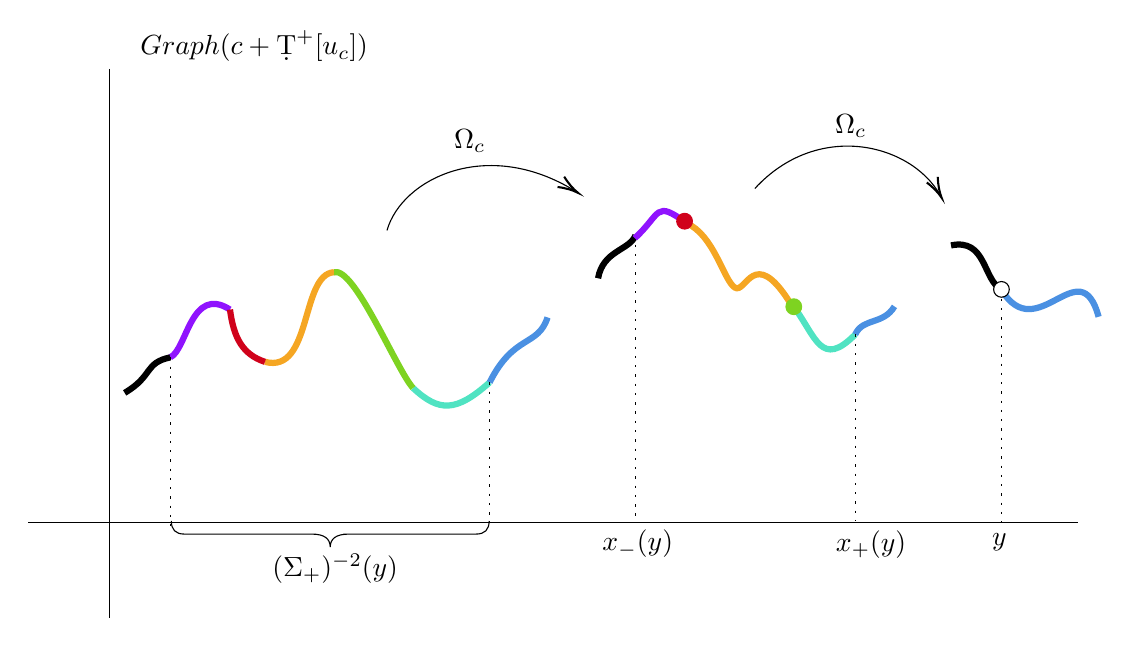
\begin{tikzpicture}[x=0.75pt,y=0.75pt,yscale=-0.9,xscale=0.9]

\draw [color={rgb, 255:red, 245; green, 166; blue, 35 }  ,draw opacity=1 ][line width=2.25]    (407.77,130.51) .. controls (422.6,137) and (427.6,161) .. (433.6,165) .. controls (439.6,169) and (443.6,142) .. (463.13,173) ;
\draw [line width=2.25]    (549.4,142.47) .. controls (568.4,138.47) and (566.4,160.93) .. (576.4,166.13) ;
\draw [color={rgb, 255:red, 74; green, 144; blue, 226 }  ,draw opacity=1 ][line width=2.25]    (576.4,166.13) .. controls (595.4,197.73) and (618.4,143.87) .. (628.4,180.67) ;
\draw  [dash pattern={on 0.84pt off 2.51pt}]  (576.4,166) -- (576.4,291.6) ;
\draw    (55.4,291) -- (617.4,291) ;
\draw    (99,48) -- (99,342) ;
\draw    (444.4,112) .. controls (477.72,75.74) and (527.37,87.5) .. (543.46,115.28) ;
\draw [shift={(544.4,117)}, rotate = 242.65] [color={rgb, 255:red, 0; green, 0; blue, 0 }  ][line width=0.75]    (10.93,-3.29) .. controls (6.95,-1.4) and (3.31,-0.3) .. (0,0) .. controls (3.31,0.3) and (6.95,1.4) .. (10.93,3.29)   ;
\draw  [color={rgb, 255:red, 0; green, 0; blue, 0 }  ,draw opacity=1 ][fill={rgb, 255:red, 255; green, 255; blue, 255 }  ,fill opacity=1 ] (572.2,166) .. controls (572.2,163.68) and (574.08,161.8) .. (576.4,161.8) .. controls (578.72,161.8) and (580.6,163.68) .. (580.6,166) .. controls (580.6,168.32) and (578.72,170.2) .. (576.4,170.2) .. controls (574.08,170.2) and (572.2,168.32) .. (572.2,166) -- cycle ;
\draw [color={rgb, 255:red, 144; green, 19; blue, 254 }  ,draw opacity=1 ][line width=2.25]    (131.4,202.4) .. controls (140.4,198.4) and (142.4,163.4) .. (163.4,176.8) ;
\draw [color={rgb, 255:red, 245; green, 166; blue, 35 }  ,draw opacity=1 ][line width=2.25]    (182.13,204.8) .. controls (207.47,211.47) and (201.13,157.8) .. (219.13,156.8) ;
\draw [color={rgb, 255:red, 80; green, 227; blue, 194 }  ,draw opacity=1 ][line width=2.25]    (261.4,218.8) .. controls (275.4,231.8) and (284.4,231.8) .. (302.4,215.8) ;
\draw [line width=2.25]    (107.01,221.4) .. controls (122.4,212.4) and (117.4,205.4) .. (131.4,202.4) ;
\draw [color={rgb, 255:red, 74; green, 144; blue, 226 }  ,draw opacity=1 ][line width=2.25]    (302.4,215.8) .. controls (315.4,189.8) and (328.4,196.8) .. (333.4,181) ;
\draw [color={rgb, 255:red, 208; green, 2; blue, 27 }  ,draw opacity=1 ][line width=2.25]    (163.4,176.8) .. controls (165.4,192) and (170.13,200.8) .. (182.13,204.8) ;
\draw [color={rgb, 255:red, 126; green, 211; blue, 33 }  ,draw opacity=1 ][line width=2.25]    (219.13,156.8) .. controls (230.13,153.8) and (252.4,208.8) .. (261.4,218.8) ;
\draw  [dash pattern={on 0.84pt off 2.51pt}]  (131.4,202.4) -- (131.4,292.53) ;
\draw  [dash pattern={on 0.84pt off 2.51pt}]  (302.4,215.8) -- (302.4,291.2) ;
\draw   (132,290) .. controls (132,294.67) and (134.33,297) .. (139,297) -- (207.07,297) .. controls (213.74,297) and (217.07,299.33) .. (217.07,304) .. controls (217.07,299.33) and (220.4,297) .. (227.07,297)(224.07,297) -- (295.13,297) .. controls (299.8,297) and (302.13,294.67) .. (302.13,290) ;
\draw    (247.47,134.4) .. controls (255.39,106.68) and (301.2,84.19) .. (348.31,113.43) ;
\draw [shift={(349.73,114.33)}, rotate = 212.74] [color={rgb, 255:red, 0; green, 0; blue, 0 }  ][line width=0.75]    (10.93,-3.29) .. controls (6.95,-1.4) and (3.31,-0.3) .. (0,0) .. controls (3.31,0.3) and (6.95,1.4) .. (10.93,3.29)   ;
\draw [color={rgb, 255:red, 80; green, 227; blue, 194 }  ,draw opacity=1 ][line width=2.25]    (465.24,175.28) .. controls (477.24,191.54) and (479.87,208.6) .. (498.13,190.13) ;
\draw  [color={rgb, 255:red, 126; green, 211; blue, 33 }  ,draw opacity=1 ][fill={rgb, 255:red, 126; green, 211; blue, 33 }  ,fill opacity=1 ] (461.43,177.04) .. controls (460.45,174.94) and (461.36,172.44) .. (463.47,171.47) .. controls (465.57,170.49) and (468.07,171.4) .. (469.04,173.51) .. controls (470.02,175.61) and (469.11,178.11) .. (467,179.09) .. controls (464.9,180.06) and (462.4,179.15) .. (461.43,177.04) -- cycle ;
\draw [line width=2.25]    (360.46,160.07) .. controls (363.06,145.07) and (377.46,145.07) .. (380.46,137.07) ;
\draw [color={rgb, 255:red, 74; green, 144; blue, 226 }  ,draw opacity=1 ][line width=2.25]    (498.13,190.13) .. controls (502.13,181.13) and (513.13,185.13) .. (519.13,175.13) ;
\draw  [dash pattern={on 0.84pt off 2.51pt}]  (380.46,137.07) -- (380.46,290.13) ;
\draw  [dash pattern={on 0.84pt off 2.51pt}]  (498.13,190.13) -- (498.13,290.13) ;
\draw [color={rgb, 255:red, 144; green, 19; blue, 254 }  ,draw opacity=1 ][line width=2.25]    (380.12,138.6) .. controls (394.6,125.2) and (390.6,118) .. (407.77,130.51) ;
\draw  [color={rgb, 255:red, 208; green, 2; blue, 27 }  ,draw opacity=1 ][fill={rgb, 255:red, 208; green, 2; blue, 27 }  ,fill opacity=1 ] (402.96,131.28) .. controls (401.98,129.17) and (402.9,126.68) .. (405,125.7) .. controls (407.1,124.72) and (409.6,125.64) .. (410.58,127.74) .. controls (411.55,129.85) and (410.64,132.34) .. (408.54,133.32) .. controls (406.43,134.3) and (403.94,133.38) .. (402.96,131.28) -- cycle ;

% Text Node
\draw (114,26.2) node [anchor=north west][inner sep=0.75pt]    {$\operatorname{Graph(} c+\d T^{+}[ u_c])$};
% Text Node
\draw (486,71.2) node [anchor=north west][inner sep=0.75pt]    {$\Omega_c$};
% Text Node
\draw (570,295.4) node [anchor=north west][inner sep=0.75pt]    {$y$};
% Text Node
\draw (361.4,293.53) node [anchor=north west][inner sep=0.75pt]    {$x_{-}( y)$};
% Text Node
\draw (486.4,293.8) node [anchor=north west][inner sep=0.75pt]    {$x_{+}( y)$};
% Text Node
\draw (184.67,306.4) node [anchor=north west][inner sep=0.75pt]    {$( \Sigma _{+})^{-2}( y)$};
% Text Node
\draw (282,79.2) node [anchor=north west][inner sep=0.75pt]    {$\Omega_c$};


\end{tikzpicture}

\end{document}